\section*{Aufgabe 1)}
\subsection*{a) und b)}
mode: test \\
pseudo\_data\_fraction: 0.9 \\
\# Die Daten werden in zwei Teile aufgespalten. Die angegebene Zahl sagt aus, wie viel Prozent der Daten als Monte Carlo verwendet werden. Der Rest sind Pseudo-Daten. \\
\\
source\_file\_moca: NeutrinoMC.root \\
roottree\_moca: Signal\_MC\_Akzeptanz \\
\# Die detektierten Signalereignisse sind im Tree: Signal\_MC\_Akzeptanz gespeichert. \\
\\
branch\_x: Energie log \\
number\_bins: 8 \\
limits\_x: 0 2 \\



\subsection*{c)}
branch\_y: AnzahlHits \\
number\_y\_bins: 0 log \\
\\
branch\_y: x \\
number\_y\_bins: 0 \\
\\
branch\_y: y \\
number\_y\_bins: 0 \\
\\
number\_all\_variables: 3 \\



\subsection*{d)}
number\_deg\_free: 15 \\
max\_number\_deg\_free: 15 \\
number\_knots: 24 \\
max\_number\_knots: 24 \\

\begin{figure}[H]
  \centering
  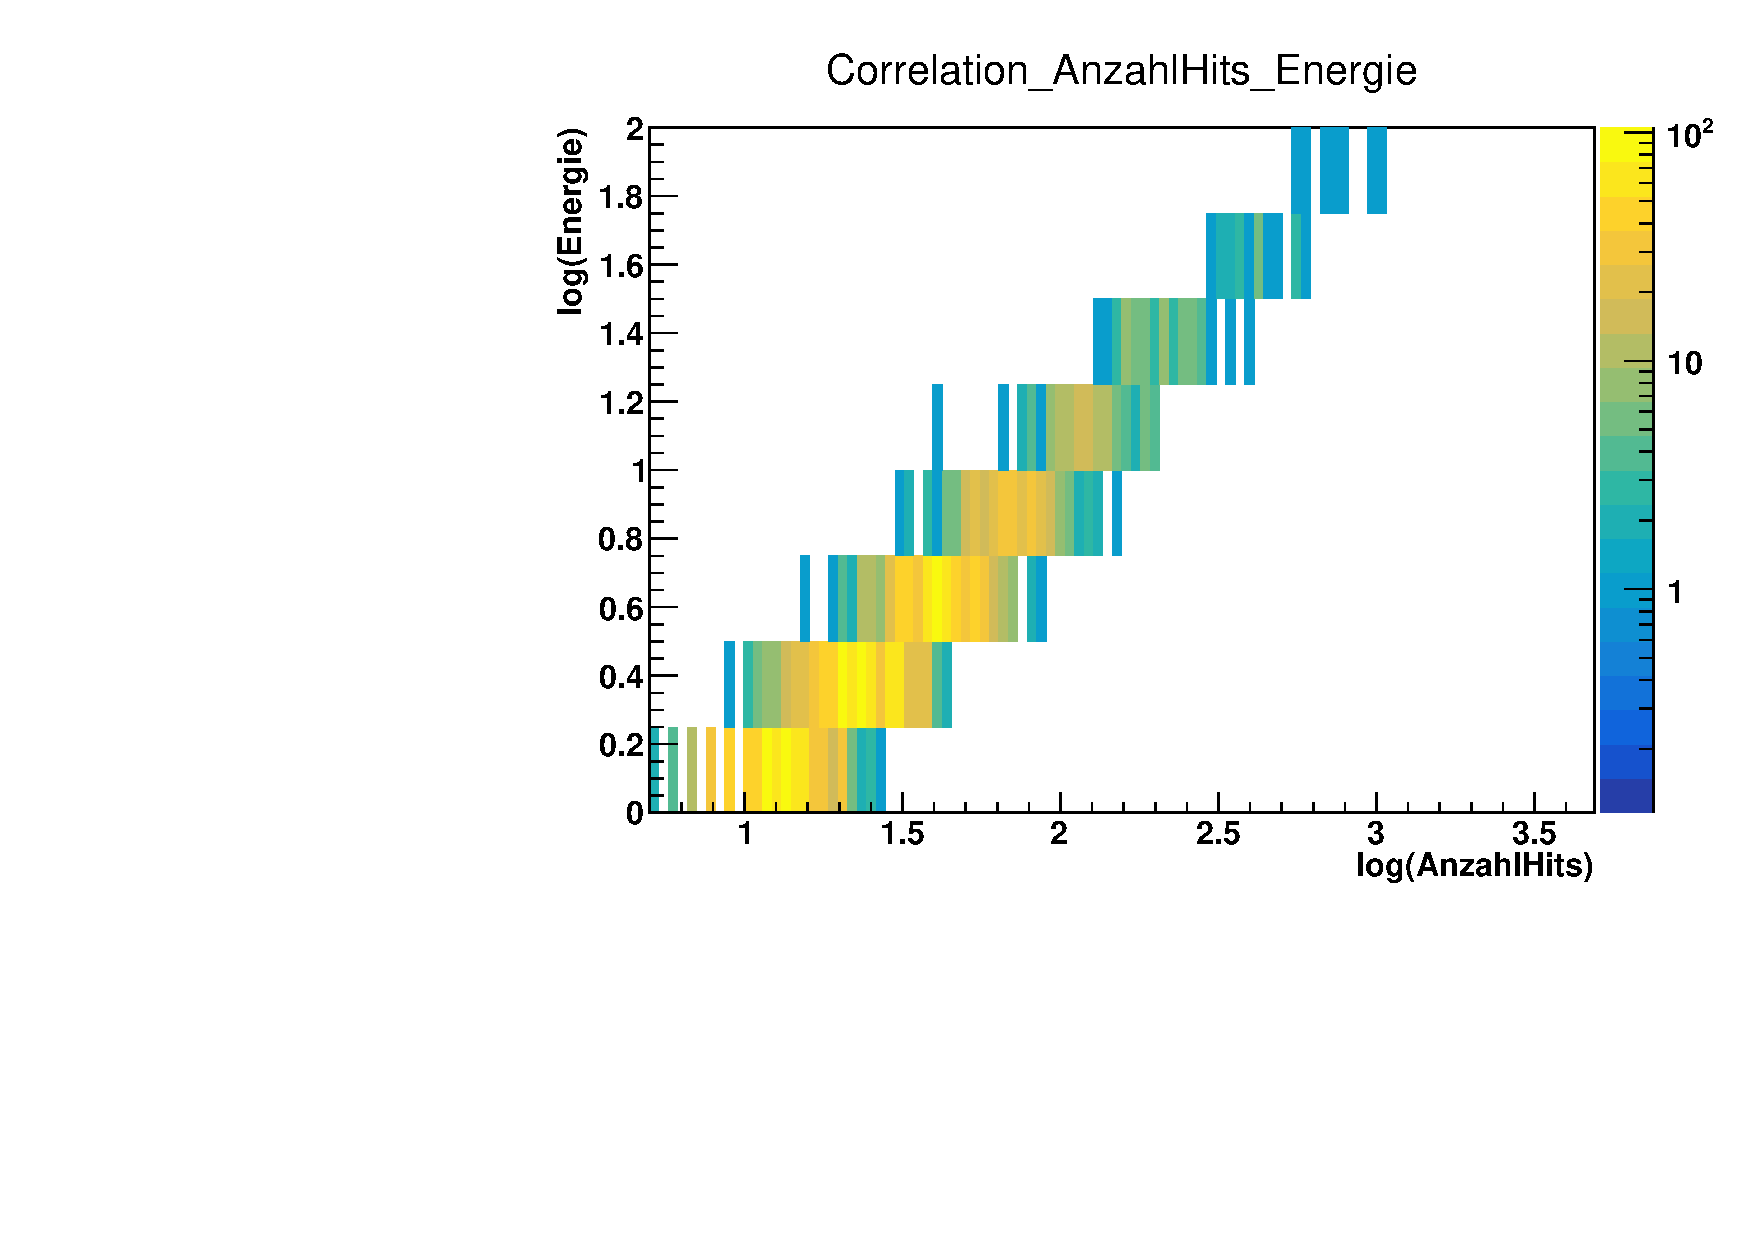
\includegraphics[height=0.4\textheight]{Bilder/CorHits.pdf}
  \caption{Korrelation zwischen Energie und Anzahlhits.}
  \label{fig:CorHits}
\end{figure}

\begin{figure}[H]
  \centering
  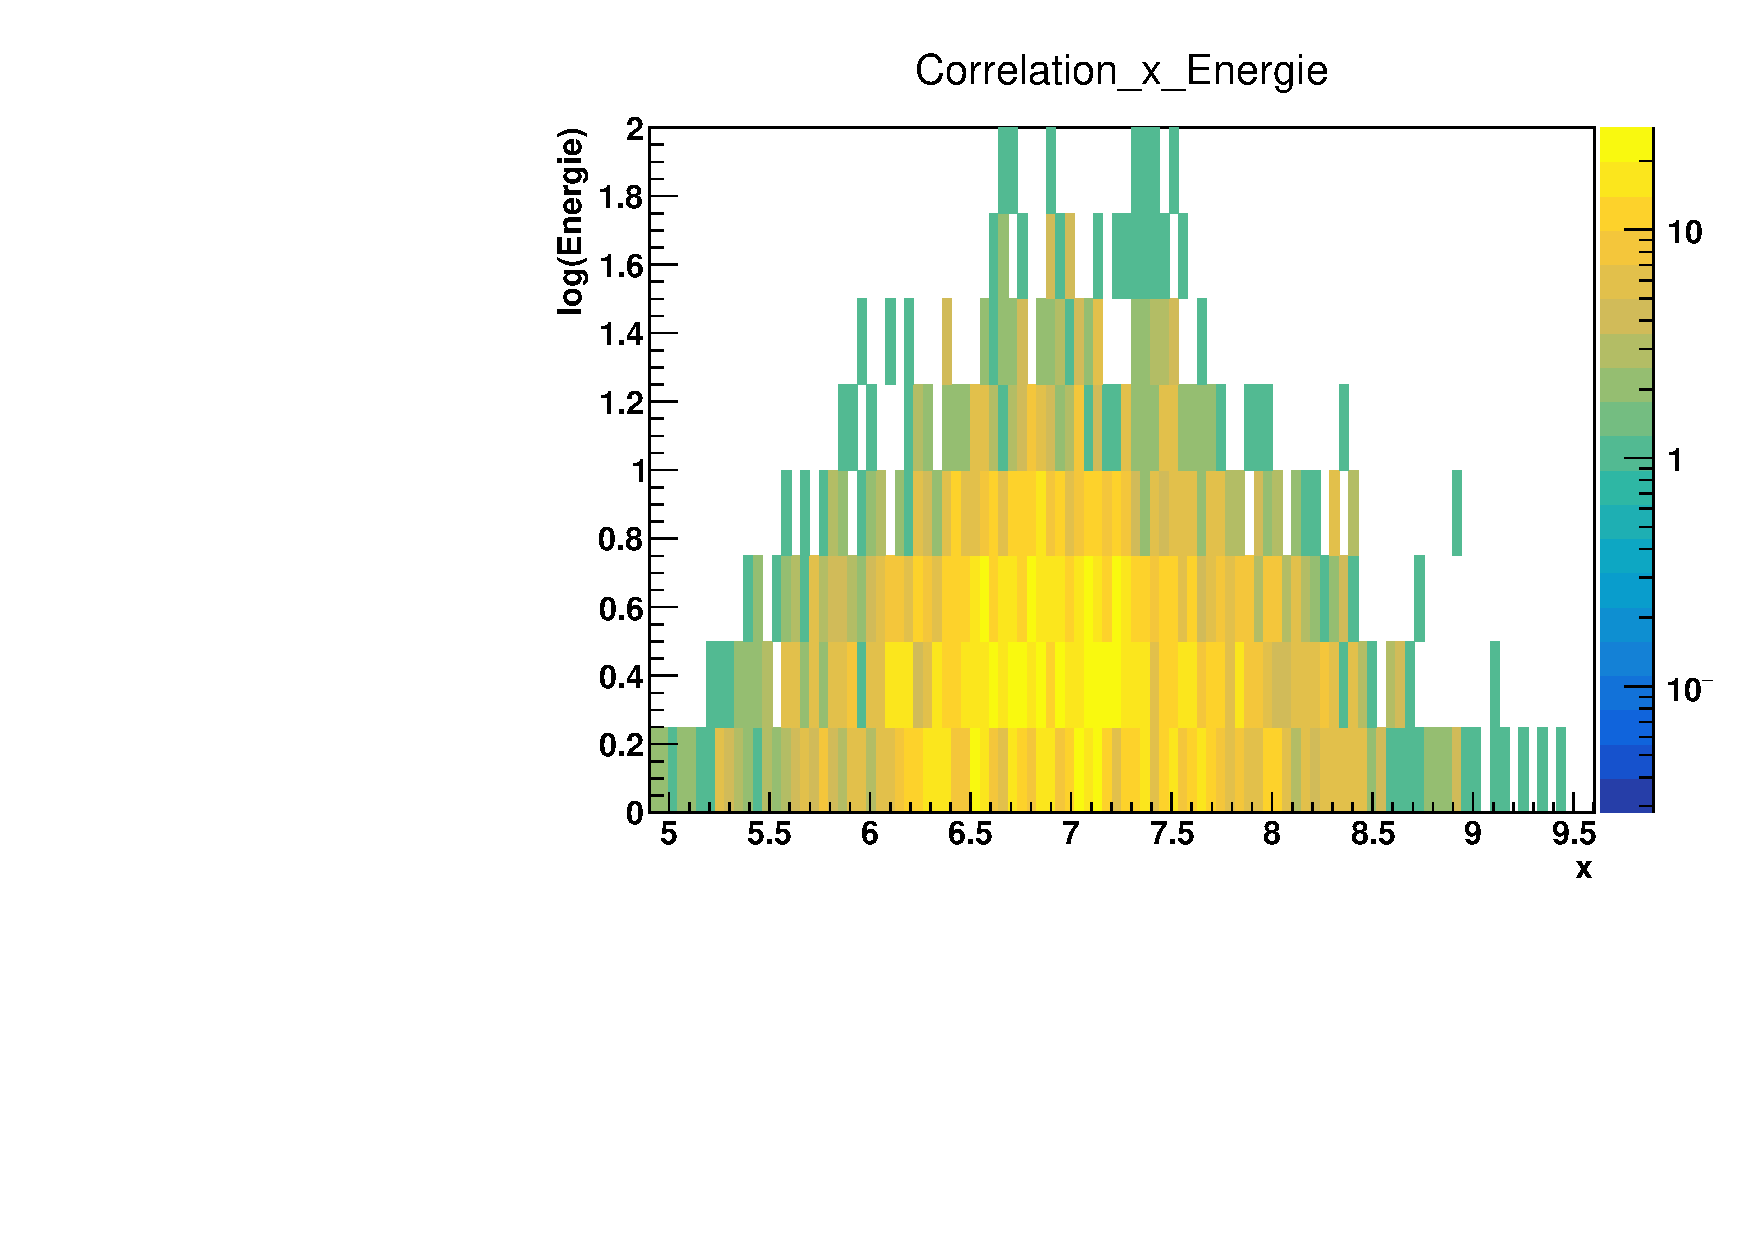
\includegraphics[height=0.4\textheight]{Bilder/CorX.pdf}
  \caption{Korrelation zwischen Energie und x.}
  \label{fig:CorX}
\end{figure}

\begin{figure}[H]
  \centering
  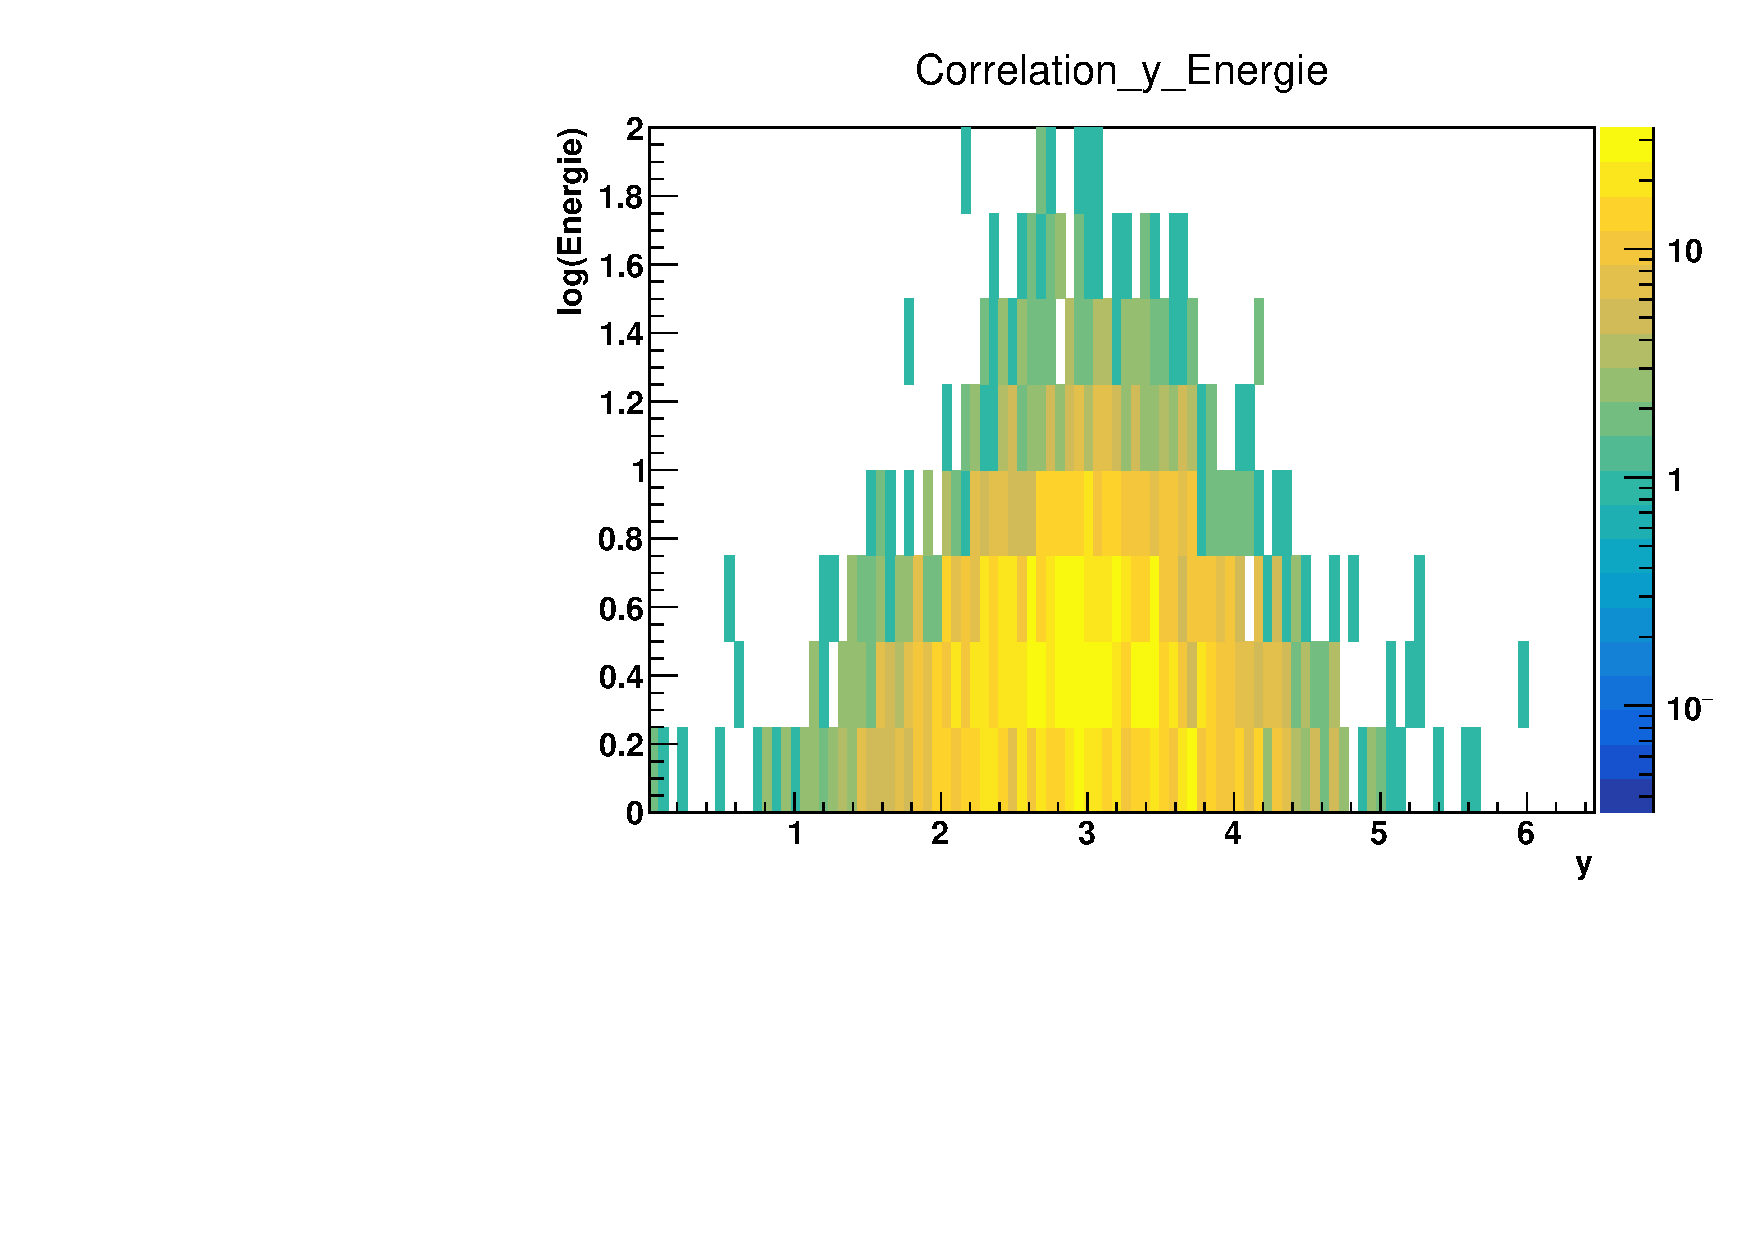
\includegraphics[height=0.4\textheight]{Bilder/CorY.pdf}
  \caption{Korrelation zwischen Energie und y.}
  \label{fig:CorY}
\end{figure}

Nein, es sind nicht alle Observablen zur Entfaltung geeignet. AnzahlHits ist am besten geeignet, weil sich eine Ellipse (eine halbe Ellipse) ausbildet. Daran kann man sehen, dass die Energie und die AnzahlHits korreliert sind. Bei den beiden anderen Plots erkennt man eher einen Kreis, deshalb sind x und y nur wenig mit der Energie korreliert.



\newpage
\subsection*{e)}
Wichtig ist, dass die "Data point correlation" (DPC) und der $\chi^2$-Test minimiert werden. Wir haben den Bereich auf ca. 24-26 Knoten und ca. 14-20 Freiheitsgrade bestimmt. Bei einer Binzahl von 8. \\
Das Testergebnis haben wir mit 8 Bins, 25 Knoten und 17 Freiheitsgraden aufgenommen, weil dort die Abweichung zwischen "true Distribution" und "unfolded distribution" am geringsten waren.

\begin{figure}
  \centering
  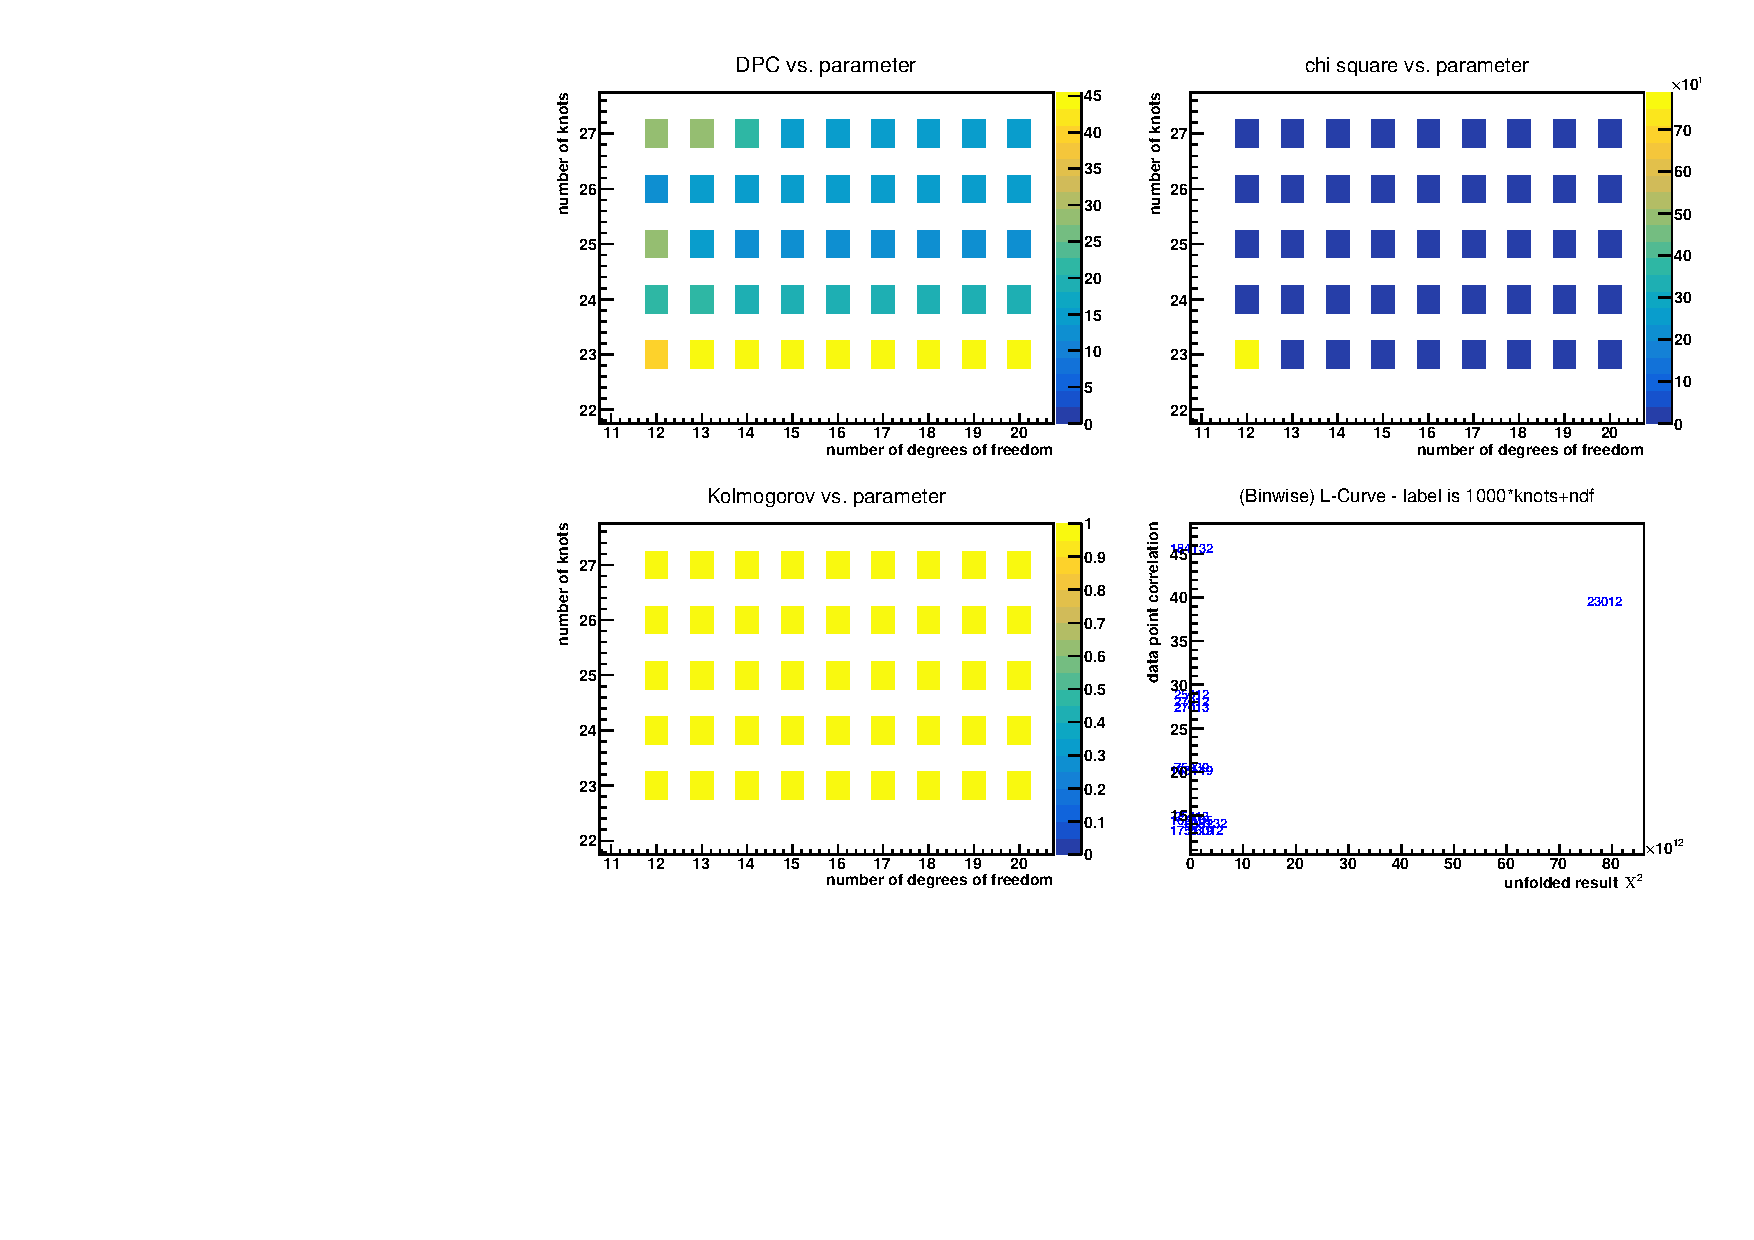
\includegraphics[width=\linewidth]{Bilder/Overview.pdf}
  \caption{DPC, $\chi^2$-Test, Kolomogorov, L-Curve gegen die Parameter}
  \label{fig:Overview}
\end{figure}

\begin{figure}
  \centering
  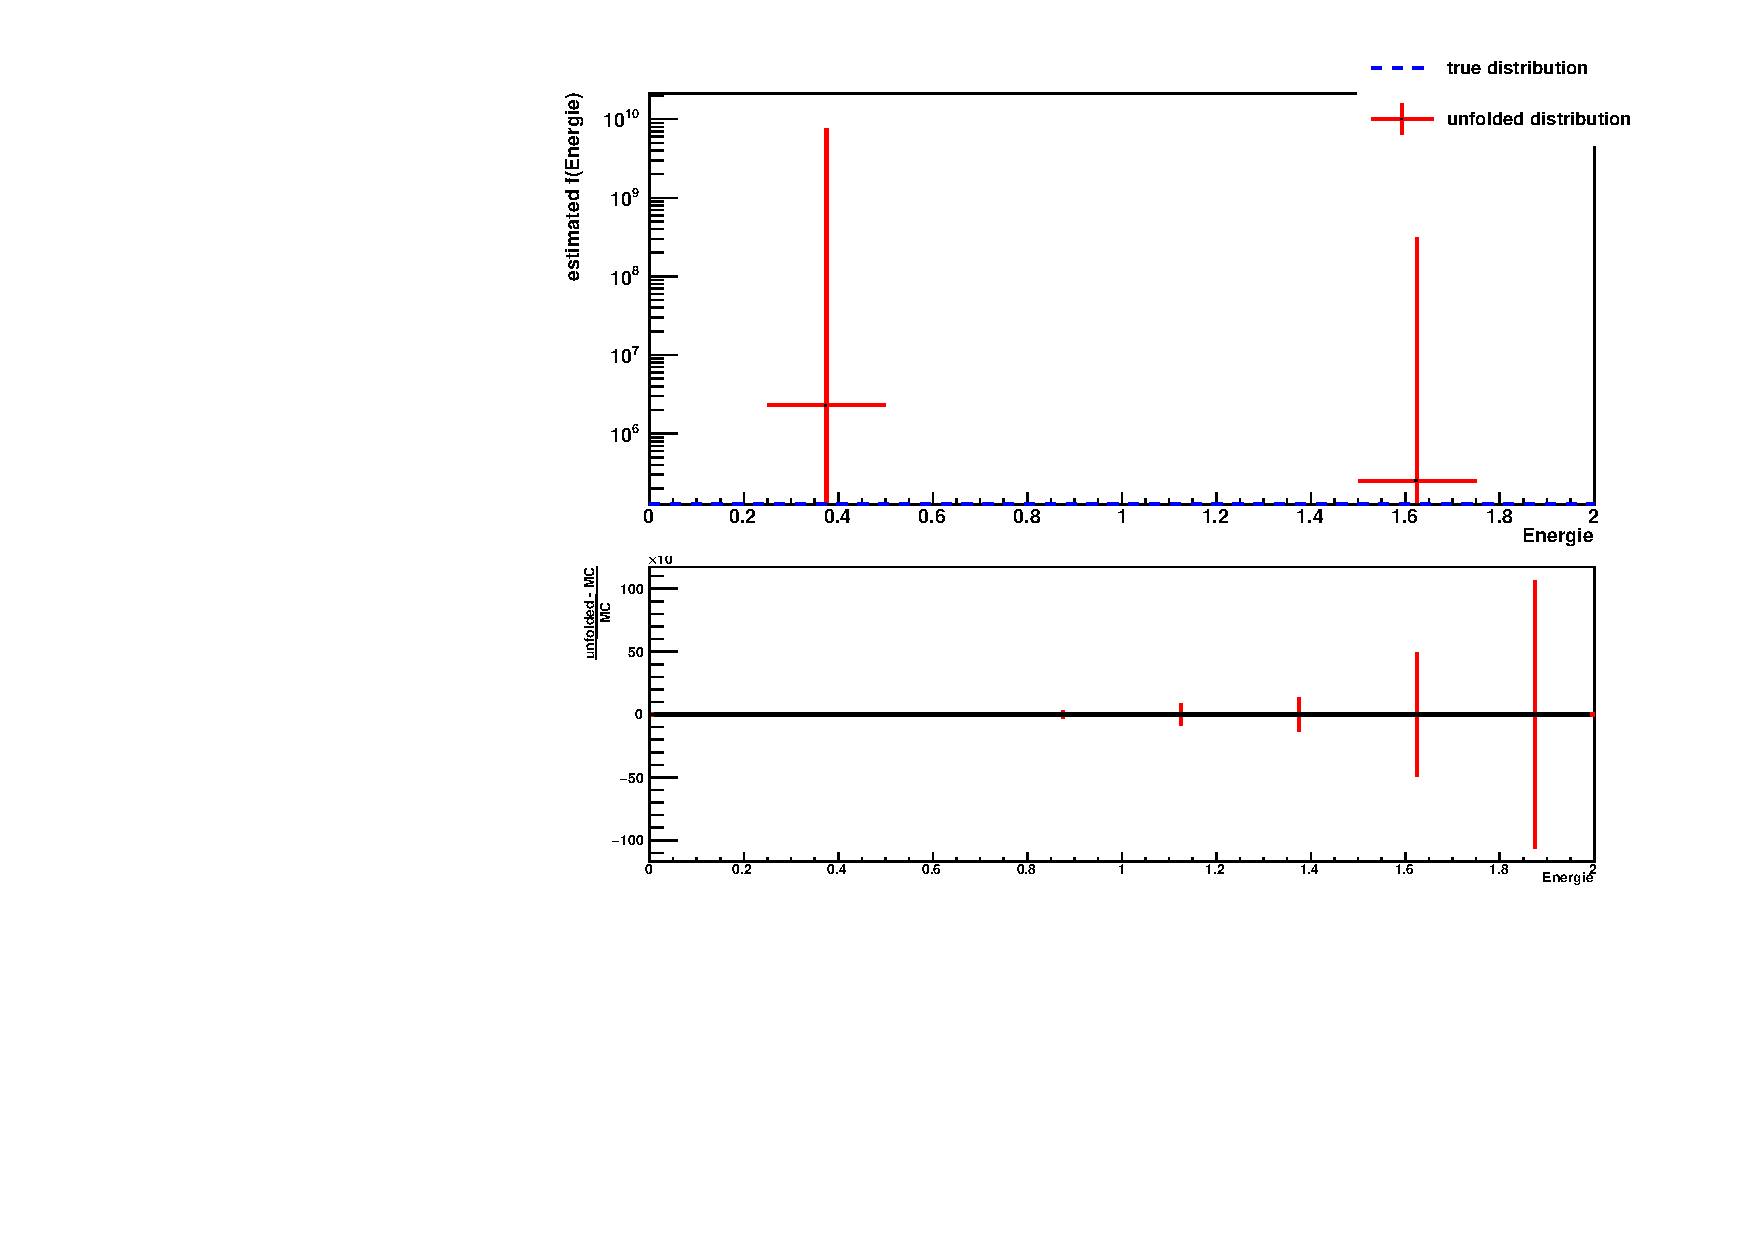
\includegraphics[width=\linewidth]{Bilder/UnfoldB8K25F17.pdf}
  \caption{Testergebnis bei 25 Knots, 17 Freiheitsgraden und 8 bins}
  \label{fig:unfold}
\end{figure}
